\chapter{Conservación de la masa.}
\section{Teorema del transporte de Reynolds.}
Se parte de una función genérica $\Phi=f(\vec{r},t) $
%\begin{figure}[H]
%	\centering
%	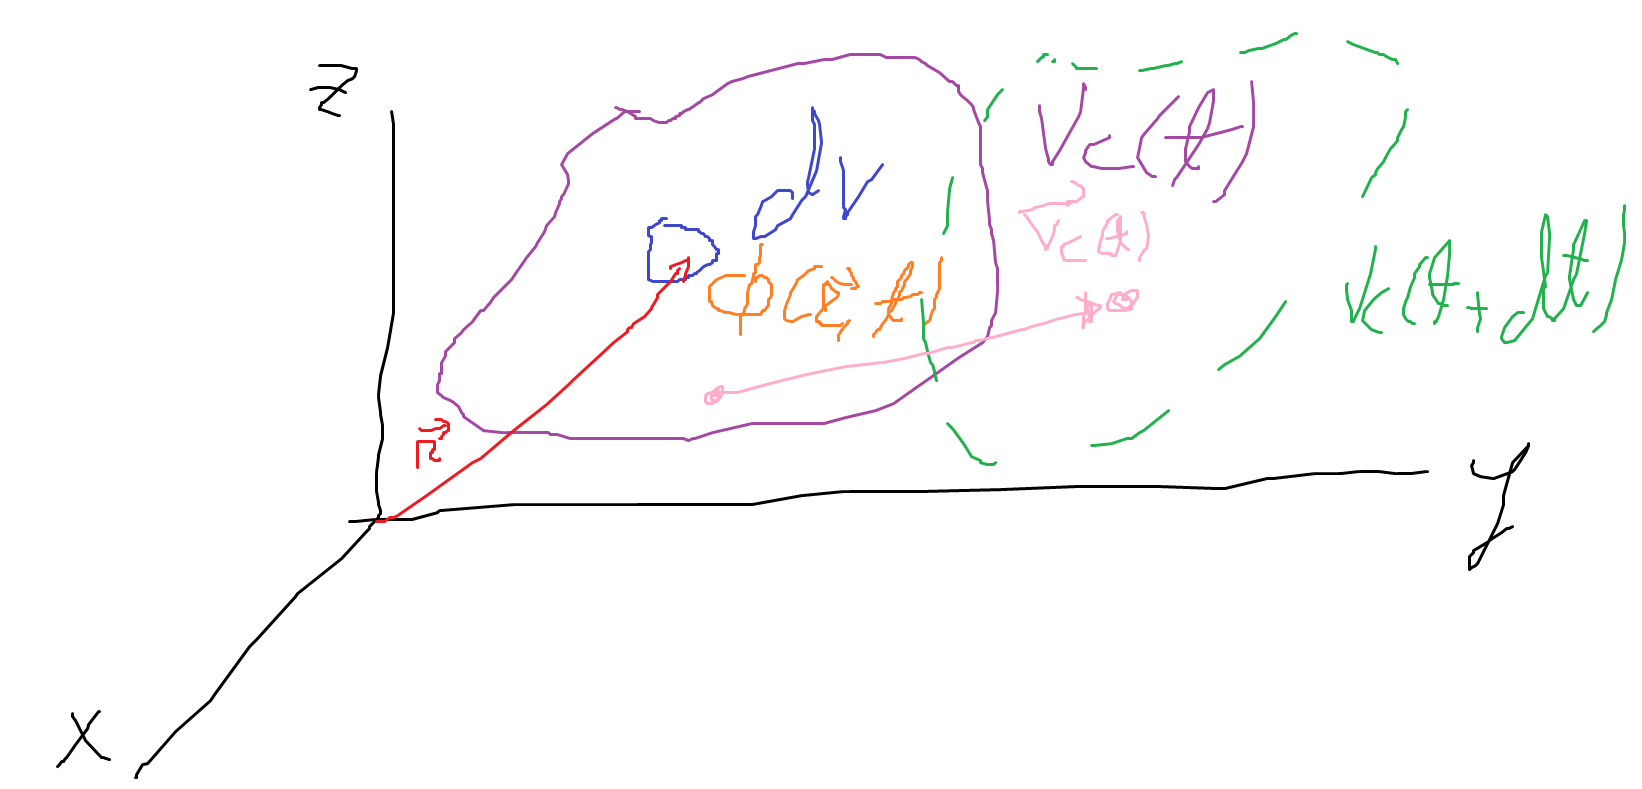
\includegraphics[width=0.7\linewidth]{imagenesTema3/magnitudesReynolds}
%	\caption{Evolución de una magnitud en un volumen fluido.}
%	\label{fig:magnitudesreynolds}
%\end{figure}

\begin{figure}[H]
	\centering
		\begin{circuitikz}
			\tikzstyle{every node}=[font=\large]
			\draw [-latex] (-1.75,15.75) -- (-1.75,21.25)node[pos=1,above]{$\vec{k}$};
			\draw [-latex] (-1.75,15.75) -- (5.75,15.75)node[pos=1,right]{$\vec{i}$};
			\draw [-latex] (-1.75,15.75) -- (-3.25,14.25)node[pos=1,left]{$\vec{j}$};
			\node [font=\large, color={rgb,255:red,128; green,0; blue,255}] at (0.5,20.75) {$V_C(t)$};
			\draw [ color={rgb,255:red,128; green,0; blue,255}, dashed] (2.25,20.25) .. controls (3,21.5) and (4,20.25) .. (5.5,20);
			\draw [ color={rgb,255:red,128; green,0; blue,255}, dashed] (5.5,20) .. controls (6.5,20) and (5.75,18.75) .. (5.75,17.5);
			\draw [ color={rgb,255:red,128; green,0; blue,255}, dashed] (5.75,17.5) .. controls (6,16) and (5,16.25) .. (3.5,16.5);
			\draw [ color={rgb,255:red,128; green,0; blue,255}, dashed] (3.5,16.5) .. controls (2.5,17) and (2,16.25) .. (1.75,17.5);
			\draw [ color={rgb,255:red,128; green,0; blue,255}, dashed] (1.75,17.5) .. controls (1.25,19) and (2,19.25) .. (2.25,20.25);
			\draw [ color={rgb,255:red,128; green,0; blue,255}, short] (-1,20.25) .. controls (0,21) and (0,19.75) .. (1,19.25);
			\draw [ color={rgb,255:red,128; green,0; blue,255}, short] (1,19.25) .. controls (2,19) and (1.5,18.5) .. (2,17.5);
			\draw [ color={rgb,255:red,128; green,0; blue,255}, short] (2,17.5) .. controls (2.5,16.5) and (1.5,16.75) .. (0.75,16);
			\draw [ color={rgb,255:red,128; green,0; blue,255}, short] (0.75,16) .. controls (-0.25,15) and (-0.25,16.25) .. (-1.25,16.25);
			\draw [ color={rgb,255:red,128; green,0; blue,255}, short] (-1.25,16.25) .. controls (-2.75,16.75) and (-1.75,17.5) .. (-2.5,18.75);
			\draw [ color={rgb,255:red,128; green,0; blue,255}, short] (-2.5,18.75) .. controls (-3,20) and (-1.75,19.5) .. (-1,20.25);
			\draw [ color={rgb,255:red,128; green,0; blue,255} ] (-0.75,19.25) circle (0.5cm);
			\draw [ color={rgb,255:red,128; green,0; blue,255}, short] (-1.25,19.25) .. controls (-1,19) and (-0.5,19) .. (-0.25,19.25);
			\draw [ color={rgb,255:red,128; green,0; blue,255}, dashed] (-1.25,19.25) .. controls (-1,19.5) and (-0.5,19.5) .. (-0.25,19.25);
			\node [font=\large, color={rgb,255:red,128; green,0; blue,255}] at (-0.5,20) {dV};
			\draw [ color={rgb,255:red,255; green,128; blue,0}, -latex] (-1.75,15.75) -- (-0.75,19.25)node[pos=0.8,left]{$\vec{r}$};
			\node [font=\large, color={rgb,255:red,128; green,0; blue,255}] at (5.25,20.5) {$V_C(t+dt)$};
			\draw [ color={rgb,255:red,0; green,128; blue,0}, -latex] (-0.75,19.25) -- (3.5,18.5)node[pos=1,above]{$\vec{v}_C(t)$};
			\node [font=\large, color={rgb,255:red,0; green,128; blue,0}] at (0.25,18.5) {$\Phi(\vec{r},$ t)};
		\end{circuitikz}
	\caption{Evolución de una magnitud en un volumen fluido.}
	\label{fig:magnitudesreynolds}
\end{figure}

Por definición de derivada:
\[\frac{d}{dt}\iiint_{V_c(t)} \Phi(\vec{r},t) \,dV=\lim_{\Delta t \to 0} \left[\iiint_{V_c(t+dt)} \Phi(\vec{r},t+dt) \,dV-\iiint_{V_c(t)} \Phi(\vec{r},t) \,dV\right]\]

Se hace el desarrollo de Taylor en t del primer término:
\[\frac{d}{dt}\iiint_{V_c(t)} \Phi(\vec{r},t) \,dV=\iiint_{V_c(t)} \frac{\partial}{\partial t}\Phi(\vec{r},t) \,dV+\lim_{\Delta t \to 0} \frac{1}{\Delta t}\left[\iiint_{V_c(t+dt)} \Phi(\vec{r},t) \,dV-\iiint_{V_c(t)} \Phi(\vec{r},t) \,dV\right]\]

Como solo se estudia la velocidad de compresión o expansión del fluido en la dirección de la superficie de control:
\[dV=\vec{v}_c\cdot\vec{n}dS\Delta t\]

Por tanto:
\begin{equation}\label{eq:ttr1}
\frac{d}{dt}\iiint_{V_c(t)} \Phi(\vec{r},t) \,dV=\iiint_{V_c(t)} \frac{\partial}{\partial t}\Phi(\vec{r},t) \,dV+\oiint_{S_c(t)} \Phi(\vec{r},t)\vec{v}_c\cdot\vec{n} \,dS
\end{equation}

De manera similar se puede aplicar esta deducción a un volumen fluido:

\begin{equation}\label{eq:ttr2}
\frac{d}{dt}\iiint_{V_f(t)} \Phi(\vec{r},t) \,dV=
\red{\underbrace{\black\iiint_{V_f(t)} \frac{\partial}{\partial t}\Phi(\vec{r},t) \,dV}_{\text{Variación local}}}
\black+
\red{\underbrace{\black\oiint_{S_f(t)} \Phi(\vec{r},t)\vec{v}\cdot\vec{n}\,dS}_{\text{Variación convectiva}}}
\black
\end{equation}

En un tiempo $t*$ paramétrico tal que $V_c(t*)=V_f(t*)$ se cumple que
\[ \iiint_{V_c(t*)}\frac{\partial \Phi}{\partial t}\,dV\approx \iiint_{V_f(t*)}\frac{\partial \Phi}{\partial t}\,dV\]

Por tanto, si se hace la siguiente resta \eqref{eq:ttr2} - \eqref{eq:ttr1}. Se obtiene el Teorema de Reynolds aplicado a los problemas:

\[\frac{d}{dt}\iiint_{V_f(t)}\Phi(\vec{r},t)\,dV=\frac{d}{dt}\iiint_{V_c(t)}\Phi(\vec{r},t)\,dV+\oiint_{S_c(t)} \Phi(\vec{r},t)\left[(\vec{v}-\vec{v}_c)\cdot\vec{n}\right] \,dS\]



Si la magnitud $\Phi = \rho$ Se obtiene la ecuación de conservación de la masa en forma integral, que como en todo el volumen fluido no varia es igual a 0:

\[\frac{d}{dt}\iiint_{V_f(t)}\rho\,dV=\frac{d}{dt}\iiint_{V_c(t)}\rho\,dV+\oiint_{S_c(t)} \rho\left[(\vec{v}-\vec{v}_c)\cdot\vec{n}\right] \,dS=0\]

Para todo el volumen fluido:
\[\frac{d}{dt}\iiint_{V_f(t)} \rho \,dV=\iiint_{V_f(t)} \frac{\partial \rho}{\partial t} \,dV+\oiint_{S_f(t)} \rho\vec{v}\cdot\vec{n} \,dS=0\]

Si $V_f(t)\approx dV_f(t)$ entonces aplicando el teorema de gauss se llega a la ecuación diferencial de la masa o forma conservativa:

\
\
\
\begin{center}
	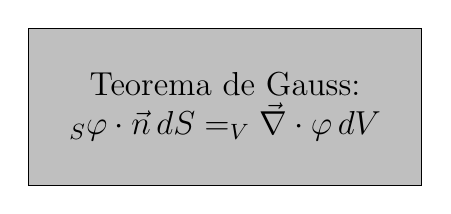
\begin{tikzpicture}
		\draw [fill=lightgray](0,0) rectangle (5, 2);
		\node at (2.5, 1) [align = center]{Teorema de Gauss: \\$\oiint_S \varphi \cdot \vec{n}\,dS=\iiint_V \vec{\nabla}\cdot\varphi\,dV $};
	\end{tikzpicture}
\end{center}

\[\lim_{dV \to 0}\left[\frac{\partial \rho}{\partial t} dV+\vec{\nabla}\cdot\left(\rho\vec{v}\right)dV\right]=0\]
\[\frac{\partial \rho}{\partial t} +\vec{\nabla}\cdot\left(\rho\vec{v}\right)=0\]
Término local de masa: 
\[\frac{\partial \rho}{\partial t}\]
Término convectivo de masa:
\[\vec{\nabla}\cdot\left(\rho\vec{v}\right)\]

\section{Flujo sobre una superficie.}
\begin{itemize}
	\item Flujo másico
	\[G_e=\iint_{S_e} \rho\left(\vec{v}-\vec{v}_c\right)\cdot\vec{n}\,dS\]
	\item Flujo volumétrico
		\[Q_e=\iint_{S_e} \left(\vec{v}-\vec{v}_c\right)\cdot\vec{n}\,dS\]
\end{itemize}

\section{Propiedades en forma diferencial.}
Partiendo de la expresión de la derivada sustancial y de la conservación de la masa en forma diferencial:
\begin{equation} \label{eq:1}
	\frac{\partial \rho}{\partial t} +\vec{\nabla}\cdot\left(\rho\vec{v}\right)=\frac{\partial \rho}{\partial t} +\left(\vec{v}\cdot\vec{\nabla}\right)\rho+\left(\vec{\nabla}\cdot\vec{v}\right)\rho=0
\end{equation}

\begin{equation} \label{eq:4}
	\frac{D \rho}{D t}=\frac{ \partial \rho}{\partial t}+\left(\vec{v}\cdot\vec{\nabla}\right)\rho
\end{equation}

Restando \eqref{eq:1} a \eqref{eq:4}:
\[\frac{D \rho}{D t}=-\left(\vec{\nabla}\cdot\vec{v}\right)\rho\]
\begin{itemize}
	\item Si $\vec{\nabla}\cdot\vec{v} =0 $ Incopresible localmente.
	\item Si $\vec{\nabla}\cdot\vec{v} >0$ Se expande localmente el diferencial de Volumen.
	\item Si $\vec{\nabla}\cdot\vec{v} <0$ Se comprime localmente el diferencial de Volumen.
\end{itemize}
